\section{Response to Reviewer \#4}

Dear Reviewer 4,\\

Thank you very much for your careful reading and constructive comments on our manuscript. Your suggestions have been invaluable in enhancing the practical relevance and technical depth of our work. We provide our detailed responses below.

\noindent\rule{17cm}{2.0pt}


%%%%%%%%%%%%%%%%%%%%%%%%%%%%%%%%%%%%%%%%%%%%%%%%%%%%%%%%%%%%%%%%%%%%%%
\subsection{Reviewer Comment-1}



\begin{mdframed}
\begin{quote}
Simplifying Assumptions in the Channel Model \\
   The paper assumes a deterministic high-Line-of-Sight (LOS) scenario for the satellite feeder link (Eq. 11), but fails to fully account for multipath effects and dynamic channel variations inherent in practical LEO satellite networks. It is recommended that the model be further refined to enhance its generalizability


\end{quote}

\end{mdframed}


\subsection{Response}

We thank the reviewer for raising this point. In the revised manuscript, three elements address this concern: (i) a clarification after Eq.~(11) in Section~II-B explains why the deterministic feeder-link model is appropriate, citing the 3GPP NTN simulation framework (TR~38.821) which treats feeder-link SNR impairments as negligible; (ii) a footnote after Eq.~(16) in Section~II-B quantifies the feeder-to-access margin (39~dB nominal, 27--34~dB under Ka-band rain) and identifies the 10~dB threshold below which the approximation degrades; and (iii) two sensitivity curves have been added to Fig.~\ref{fig:prop1_validation} showing BLER loss less than 1.5~dB when the margin exceeds 10~dB, with significant degradation appearing only in regimes typically mitigated by gateway diversity. Multipath and dynamic channel variations are fully accounted for on the access link through the Rician fading model, SINR impairment model, and finite-blocklength BLER analysis. The deterministic feeder-link assumption is standard in the 3GPP NTN channel model (TR~38.811~\cite{3GPP_TR38811}) and is justified by the physical characteristics of the gateway--satellite link. The gateway antenna operates in a clear-sky environment with a direct view of the satellite, and the large dish aperture ($>$5~m) provides a narrow beamwidth that spatially filters any ground-reflected components. The dominant atmospheric impairment on the feeder link is Ka-band rain attenuation. A footnote after~\eqref{eq:combined_snr_final} quantifies this margin:

\begin{quote}
``{\color{blue}Under the parameters in Table~\ref{tab:sim_params}, the ratio $\bar{\gamma}_{i,\mathrm{GS}}/\bar{\gamma}_{i,\mathrm{SU}}$ exceeds 39~dB. According to ITU-R P.618~\cite{ITU-R_P618-14}, Ka-band rain attenuation at 99.9\% link availability for mid-latitude gateway sites is typically 5--12~dB, which reduces this margin to approximately 27--34~dB, well above the 10~dB threshold at which the approximation begins to degrade. The sensitivity of the subchannel BLER to reduced $\bar{\gamma}_{i,\mathrm{GS}}/\bar{\gamma}_{i,\mathrm{SU}}$ is quantified in Fig.~\ref{fig:prop1_validation}.}''
\end{quote}

The following discussion has been added to Section~V:

\begin{quote}
``{\color{blue}Fig.~\ref{fig:prop1_validation} also evaluates the sensitivity of the subchannel BLER to feeder-link degradation by showing simulation results for $n_c = 256$ with reduced feeder-to-access SNR margins of $\bar{\gamma}_{i,\mathrm{GS}}/\bar{\gamma}_{i,\mathrm{SU}} = 10$~dB and $3$~dB, corresponding to severe and extreme Ka-band rain fade conditions, respectively. The BLER loss is less than 1.5~dB when $\bar{\gamma}_{i,\mathrm{GS}}/\bar{\gamma}_{i,\mathrm{SU}}$ exceeds 10~dB, while significant degradation appears only when $\bar{\gamma}_{i,\mathrm{GS}}/\bar{\gamma}_{i,\mathrm{SU}}$ falls below 10~dB, a regime that corresponds to rain attenuation exceeding 30~dB and is typically mitigated through gateway diversity in operational systems.}''
\end{quote}

\begin{center}
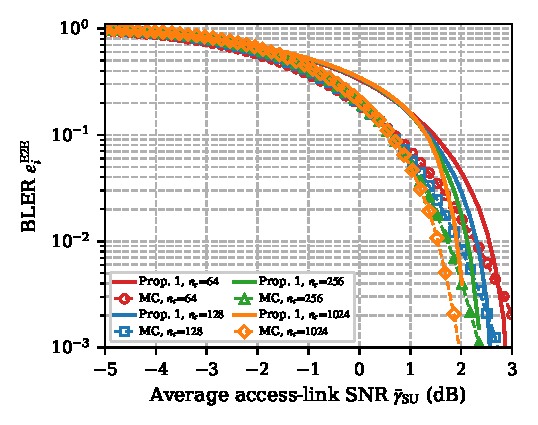
\includegraphics[width=0.7\columnwidth]{prop1_closedform_validation.eps}\\
{\small \textbf{Fig.~\ref{fig:prop1_validation}:} Subchannel BLER versus average access-link SNR for different blocklengths $n_c$ under dominant-LOS Rician fading. {\color{blue}Feeder-link sensitivity is shown for $n_c = 256$ with $\bar{\gamma}_{i,\mathrm{GS}}/\bar{\gamma}_{i,\mathrm{SU}} = 10$~dB and $3$~dB.}}
\end{center}

We trust that the added clarification, sensitivity curves, and supporting evidence demonstrate the generalisability of the channel model.


\subsection{Reviewer Comment-2}



\begin{mdframed}
\begin{quote}
Construction Method of Diversity Transform \\
   While the manuscript mentions constructing the diversity transform matrix based on Reed-Solomon codes, it lacks a detailed discussion on the performance trade-offs regarding finite code lengths and practical channels. I suggest adding a discussion on construction complexity and decoding latency.


\end{quote}

\end{mdframed}


\subsection{Response}

We thank the reviewer for this suggestion. A new subsection, Section~IV-F, ``Implementation Complexity,'' has been added to the revised manuscript, covering four aspects: encoding/decoding complexity ($O(\varrho \cdot n_{\mathrm{out}} \cdot n_c)$ binary additions, negligible versus the $O(\varrho \cdot L \cdot N \log N)$ SCL cost), offline transform construction with precomputed recovery matrices, memory footprint (polynomial in MDS parameters), and signalling overhead (at most $\lceil\log_2\binom{n_{\mathrm{s}}}{k_{\mathrm{c}}}\rceil$ bits per frame). Regarding finite code length trade-offs, the MDS construction guarantees recovery for any $k_{\mathrm{c}}$ surviving blocks regardless of blocklength; the finite-blocklength penalty manifests in the per-subchannel polar code BLER, validated across $n_c = 64$ to $1024$ in Fig.~\ref{fig:prop1_validation}. A new FEC comparison (Fig.~\ref{fig:fec_comparison}) further confirms FEC-agnostic operation with polar and LDPC codes at three code rates. In the revised manuscript:

\begin{quote}
``{\color{blue}\textbf{Encoding and Decoding Complexity.}
At the transmitter, the diversity mapper computes
$\mathbf{Z} = G_{\mathrm{DIV}}^{\mathsf{T}}\,\mathbf{X}$, where
$\mathbf{X} \in \mathbb{F}_2^{\varrho \times n_c}$ contains the
$\varrho$ polar-encoded subwords. Since $G_{\mathrm{DIV}}$ is binary,
each entry of $\mathbf{Z}$ is obtained by XOR-ing at most $\varrho$
bits, yielding a total of
$O(\varrho \cdot n_{\mathrm{out}} \cdot n_c)$ binary additions.
At the receiver, diversity demapping applies a precomputed binary
recovery matrix
$G_{\mathrm{DIV}}^{\dagger}(E^c) \in
\mathbb{F}_2^{\varrho \times |E^c|}$
at the same asymptotic cost. For $n_c = N$, the diversity layer cost
$O(\varrho\, n_{\mathrm{out}}\, N)$ is typically much smaller than
the total SCL decoding cost $O(\varrho\, L\, N \log N)$, since
$L \log N \gg n_{\mathrm{out}}$ in practical settings. Consequently, the diversity demapping adds negligible
processing latency to the decoding pipeline, preserving the
single-pass receiver architecture described in
Section~\ref{subsec:receiver_demapping}.}

{\color{blue}\textbf{Transform Construction and Update Overhead.}
The RS--Vandermonde construction in
Algorithm~\ref{alg:div_transform_construction} requires
$O(k_{\mathrm{c}} \cdot n_{\mathrm{s}} \cdot m^2)$ finite-field
multiplications to build $G_{\mathrm{MDS}}$ and compute the faithful
binary representation. This computation is executed once offline,
together with all $\binom{n_{\mathrm{s}}}{k_{\mathrm{c}}}$ recovery
matrices, one per admissible erasure pattern, which are stored in a
lookup table.
Since the MDS code parameters $(k_{\mathrm{c}}, n_{\mathrm{s}}, m)$
are fixed for a given system configuration, the matrix
$G_{\mathrm{DIV}}$ itself remains static across frames.
At each frame, the ephemeris-driven predictor in
Section~\ref{sec:ephemeris_prediction} computes per-subchannel
BLER estimates $\tilde{\epsilon}_{i}^{\mathrm{E2E}}$ and
identifies which subchannels exceed the erasure threshold
$\epsilon_{\mathrm{th}}$, producing the predicted outage set
$S_{\mathrm{out}}$ in~\eqref{eq:outage_set}. The receiver then
selects the corresponding precomputed recovery matrix from the
lookup table indexed by $S_{\mathrm{out}}$. Thus, the only
per-frame update is a table index selection, not a matrix
recomputation.}

{\color{blue}\textbf{Memory Footprint.}
The binary diversity transform matrix
$G_{\mathrm{DIV}} \in \mathbb{F}_2^{\varrho \times n_{\mathrm{out}}}$
requires $\varrho \cdot n_{\mathrm{out}}$ bits of storage.
The precomputed recovery matrices, one for each of the
$\binom{n_{\mathrm{s}}}{k_{\mathrm{c}}}$ erasure patterns and
each of size $\varrho \times \varrho$ bits, add
$\binom{n_{\mathrm{s}}}{k_{\mathrm{c}}} \cdot \varrho^2$ bits.
Both quantities scale polynomially in the MDS code parameters and
are negligible compared to the $O(L \cdot N)$ bits required for
SCL decoding path storage.}

{\color{blue}\textbf{Signalling Overhead.}
The diversity transform is determined by the MDS code parameters
$(k_{\mathrm{c}}, n_{\mathrm{s}}, m)$ and the predicted erasure
family $\mathcal{E}_{\mathrm{robust}}$. Since both the gateway
and the UE share ephemeris data
(Section~\ref{sec:ephemeris_prediction}), the erasure family can
be independently computed at both ends without explicit signalling.
In operational scenarios where signalling is preferred for
robustness, the active erasure pattern index requires at most
$\lceil\log_2\binom{n_{\mathrm{s}}}{k_{\mathrm{c}}}\rceil$ bits
per OTFS frame, which is negligible relative to the $n_c$ coded
symbols transmitted per subchannel.}''
\end{quote}

Regarding performance trade-offs for finite code lengths, the MDS construction guarantees that any $k_{\mathrm{c}}$ out of $n_{\mathrm{s}}$ surviving subchannel blocks preserve full rank (Theorem~\ref{thm:block_mds}), regardless of the code length. The finite-blocklength penalty manifests in the per-subchannel polar code BLER, which is captured by Proposition~\ref{prop:bler_approx} and validated in Fig.~\ref{fig:prop1_validation} across blocklengths from $n_c = 64$ to $1024$. The diversity transform operates at the block level and is therefore independent of the per-subchannel coding blocklength. The blocklength trade-off is quantified in Fig.~\ref{fig:bler_vs_blocklength}. In Section~\ref{sec:results}:

\begin{quote}
``Fig.~\ref{fig:bler_vs_blocklength} examines how the system BLER varies with the codeword blocklength $N$ at a fixed rate $R_c = 0.5$. The BLER decreases with $N$ for all schemes, as longer codes provide greater error‑correction capability. The diversity transform maintains a consistent advantage across all blocklengths, with the largest relative gain at short blocklengths, where the standalone polar code is most susceptible to deep fades on individual subchannels. As $N$ increases, the performance gap narrows because the stronger polar code can independently recover from moderate fading without the diversity layer.''
\end{quote}

\begin{center}
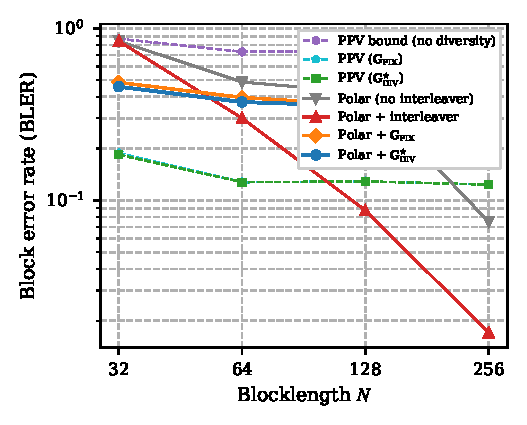
\includegraphics[width=0.7\columnwidth]{bler_vs_blocklength.eps}\\
{\small \textbf{Fig.~\ref{fig:bler_vs_blocklength}:} System BLER versus polar code blocklength $N$ at $P_{\mathrm{total}} = 10$~dBW.}
\end{center}

To further demonstrate that the framework is not restricted to a specific FEC scheme, a new FEC comparison figure has been added. In Section~\ref{sec:results}:

\begin{quote}
``{\color{blue}Fig.~\ref{fig:fec_comparison} demonstrates the FEC-agnostic operation of the proposed diversity transform by comparing polar codes (SCL decoding, list size~$32$) and LDPC codes (BP decoding, $50$ iterations) at three code rates $R_c \approx 1/4$, $1/2$, and $3/4$. All codes are combined with the diversity transform $\mathbf{G}_{\mathrm{DIV}}$ and evaluated under identical channel conditions. At each code rate, the polar and LDPC curves are nearly indistinguishable, with the residual gap remaining below $0.2$~dB across the entire power range. This confirms that the system BLER is dominated by the diversity transform's erasure recovery mechanism rather than by the specific FEC decoder, confirming FEC-agnostic operation. The diversity gain is largest at higher code rates: at $R_c = 3/4$, the no-diversity baseline remains above $0.25$ even at $P_{\mathrm{total}} = 23$~dBW, whereas the diversity-transform-equipped schemes reach $0.03$, because the weaker FEC protection makes the system more reliant on the erasure recovery provided by $\mathbf{G}_{\mathrm{DIV}}$. At $R_c = 1/4$, the stronger FEC narrows the gap, but the diversity transform still provides a consistent advantage across all power levels.}''
\end{quote}

\begin{center}
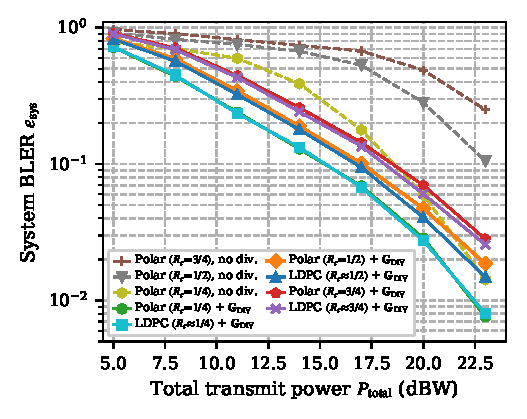
\includegraphics[width=0.7\columnwidth]{fec_comparison.eps}\\
{\small \textbf{Fig.~\ref{fig:fec_comparison}:} {\color{blue}System BLER versus total transmit power for polar and LDPC codes with the proposed diversity transform. No-diversity baselines shown for reference.}}
\end{center}

We trust that the new complexity subsection, blocklength analysis, and FEC comparison provide the practical assessment requested.


\subsection{Reviewer Comment-3}



\begin{mdframed}
\begin{quote}
Applicability of Finite Blocklength Analysis \\
   The finite blocklength analysis provided focuses primarily on OTFS performance over Rician fading channels but does not extend to broader fading models (e.g., Nakagami-m). It would be beneficial to include comparative experiments in the simulation section.

\end{quote}

\end{mdframed}


\subsection{Response}

We thank the reviewer for this suggestion. The finite-blocklength BLER framework in the paper is general and not restricted to Rician fading. In the revised manuscript, a clarifying footnote after Theorem~\ref{thm:fbl_bler} in Section~III-A makes this explicit: the expectation in the BLER expression applies to any fading distribution through the CDF of the combined SNR, and the Rician-to-Nakagami-$m$ mapping $m = (K+1)^2/(2K+1)$ is stated. The paper already validates two fading regimes spanning the practical range: dominant-LOS Rician fading ($K = 2$, $m \approx 1.8$) in Fig.~\ref{fig:prop1_validation} and pure Rayleigh fading ($K = 0$, $m = 1$) in Fig.~\ref{fig:prop2_diversity}. The Rician model is adopted because it is specified by the 3GPP NTN channel model (TR~38.811) and has a clear physical interpretation for LEO satellite--UE links. In the revised manuscript:

\begin{quote}
``{\color{blue}The expectation in~\eqref{eq:bler_exact} is general and applies to any fading distribution through the CDF of the combined SNR $\gamma_i^{\mathrm{c}}$.}''

Footnote: ``{\color{blue}For Nakagami-$m$ fading, the CDF is the regularised lower incomplete gamma function $\Upsilon(m, \gamma/\bar{\gamma})$, and substituting this CDF into~\eqref{eq:bler_exact} recovers the Nakagami-$m$ FBL BLER directly. The Rician and Nakagami-$m$ distributions are related by $m = (K_{i,k\ell}+1)^2/(2K_{i,k\ell}+1)$; setting $K_{i,k\ell} = 0$ yields Rayleigh fading ($m = 1$), as shown in Corollary~\ref{cor:bler_rayleigh}.}''
\end{quote}

Theorem~\ref{thm:fbl_bler} computes the average BLER as an expectation over the combined SNR distribution, and the underlying PPV normal approximation does not depend on the fading model. The Rician channel model is used to derive the specific closed-form expressions in Proposition~\ref{prop:bler_approx} and Corollary~\ref{cor:bler_rayleigh}, but the Nakagami-$m$ distribution is encompassed through the well-known mapping $m = (K_{i,k\ell}+1)^2/(2K_{i,k\ell}+1)$. For any desired Nakagami-$m$ parameter, one can compute the equivalent Rician K-factor and evaluate the BLER using the existing expressions.

The paper already validates two fading regimes that span the practical range for LEO satellite channels. Fig.~\ref{fig:prop1_validation} validates the closed-form BLER from Proposition~\ref{prop:bler_approx} against simulation under dominant-LOS Rician fading with $K = 2$ ($m \approx 1.8$) across blocklengths $n_c = 64$ to $1024$. Fig.~\ref{fig:prop2_diversity} validates Corollary~\ref{cor:bler_rayleigh} under pure Rayleigh fading ($K = 0$, equivalent to Nakagami-$m = 1$) for different DD diversity orders $L = 1, 2, 4, 8$, including the high-SNR asymptotic from Proposition~\ref{prop:bler_high_snr}. Together, these two figures cover the range from $m = 1$ (Rayleigh/NLOS-dominated) to $m \approx 1.8$ (moderate LOS).

\begin{center}
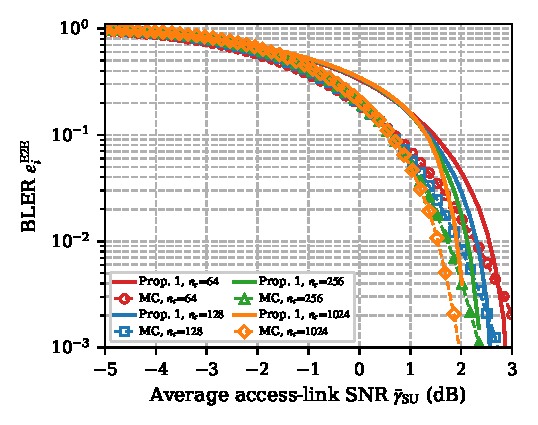
\includegraphics[width=0.7\columnwidth]{prop1_closedform_validation.eps}\\
{\small \textbf{Fig.~\ref{fig:prop1_validation}:} Subchannel BLER versus average access-link SNR under dominant-LOS Rician fading ($K = 2$, $m \approx 1.8$): simulation and closed-form approximation from Proposition~\ref{prop:bler_approx}.}
\end{center}

\begin{center}
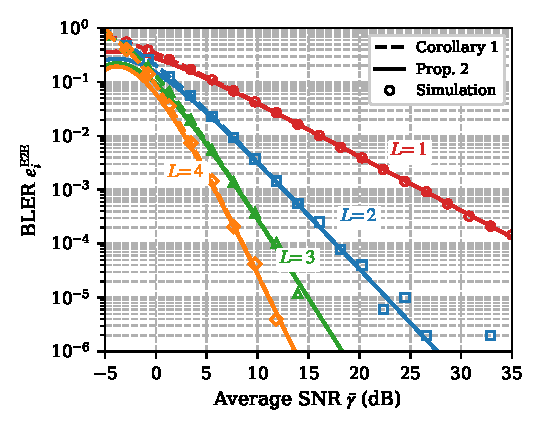
\includegraphics[width=0.7\columnwidth]{prop2_diversity_order.eps}\\
{\small \textbf{Fig.~\ref{fig:prop2_diversity}:} Subchannel BLER versus average access-link SNR under pure Rayleigh fading ($K = 0$, Nakagami-$m = 1$) for different DD diversity orders $L$: simulation, closed-form from Corollary~\ref{cor:bler_rayleigh}, and high-SNR asymptotic from Proposition~\ref{prop:bler_high_snr}.}
\end{center}

The choice of Rician fading for the access link is motivated by the 3GPP NTN channel model (TR~38.811~\cite{3GPP_TR38811}), which specifies a dominant LOS component with elevation-dependent K-factor for satellite--UE links. For LEO satellite channels where the LOS/NLOS decomposition has a clear physical interpretation (direct path versus local scattering at the UE), the Rician model is more physically accurate and is the standard choice in the satellite communications literature. The Nakagami-$m$ model would produce equivalent results at the corresponding $m$ values through the $K$-to-$m$ mapping.

We trust that this clarification demonstrates the generality of the finite-blocklength framework.


\subsection{Reviewer Comment-4}



\begin{mdframed}
\begin{quote}

Completeness of Simulation Verification \\
   Although the simulation results demonstrate improvements in BLER and latency, the specific parameter settings (such as detailed channel coding parameters and OTFS frame structure) are not clearly described. Please supplement these details to ensure the reproducibility of the results.

\end{quote}

\end{mdframed}


\subsection{Response}

We thank the reviewer for this comment. In the revised manuscript, Table~\ref{tab:sim_params} in Section~V has been expanded to include all parameters required for full reproducibility: channel coding parameters (polar code $(256,128)$, SCL list size~8), OTFS frame structure ($16 \times 64$ DD grid, QPSK, frame duration $\approx 1.07$~ms), MDS code configuration ($(k_{\mathrm{c}}, n_{\mathrm{s}}, m) = (4,6,3)$), and all system-level settings including HARQ-CC parameters. Each figure caption explicitly states which parameters differ from the defaults. The updated table is reproduced below:

\begin{center}
\begin{tabular}{@{}ll@{}}
\toprule
\textbf{Parameter} & \textbf{Value} \\
\midrule
Orbital altitude $h_{\mathrm{orb}}$ & 600~km \\
Feeder-link / access-link frequency & 20~GHz / 2~GHz \\
System bandwidth & 5~MHz \\
Subcarrier spacing $\Delta f$ & 15~kHz \\
Gateway Tx / Rx antenna gain $\mathcal{G}_G$ & 50~dBi / 35~dBi \\
Satellite Tx $\mathcal{G}_S$ / UE Rx $\mathcal{G}_U$ & 30~dBi / 0~dBi \\
OTFS modulation (QPSK, $N_{\mathrm{D}} \times M_{\mathrm{D}}$) & $16 \times 64$ \\
TDL--D taps $L_i$ / relative powers & 2 / $[0, -3]$~dB \\
Rician K-factor $K_{i,\mathrm{SU}}$ & 3.0~dB \\
Shadow fading $(\mu_{\mathrm{sh}}, \sigma_{\mathrm{sh}})$ & $(3, 4)$~dB \\
Deep blockage loss $\mathcal{L}_{\mathrm{deep}}$ & 20~dB \\
Polar code $(N, K)$ / rate $R_c$ & $(256, 128)$ / $0.5$ \\
Decoder & SCL ($L = 8$) \\
MDS parameters $(k_{\mathrm{c}}, n_{\mathrm{s}}, m)$ & $(4, 6, 3)$ \\
Diversity dimensions $(\varrho, n_{\text{out}})$ & $(12, 18)$ \\
Minimum distance $d_{\min}$ & 3 \\
LEO round-trip time  & 20~ms \\
Erasure threshold $\epsilon_{\mathrm{th}}$ & 0.1 \\
Noise power $\sigma_{n,S}^2$ / $\sigma_{n,U}^2$ & $-130.7$ / $-126.7$~dBW \\
Elevation angle $\epsilon$ & $50^{\circ}$ \\
{\color{blue}Subchannel elevation spread} & {\color{blue}$30^{\circ}$} \\
Total transmit power $P_{\mathrm{total}}$ & 8~dBW \\
Number of subchannels $n_{\mathrm{s}}$ & 6 \\
{\color{blue}HARQ-CC max retransmissions $K_{\max}$} & {\color{blue}4} \\
\bottomrule
\end{tabular}
\end{center}

The OTFS frame structure is fully specified by these parameters. The ISFFT and Heisenberg transform mapping from the DD domain to the time--frequency domain is described in Section~II-C, with the DD-domain input--output relation given by~\eqref{eq:dd_io}. The frame duration is $T_{\mathrm{frame}} = n_c / (M_{\mathrm{D}} \Delta f) = 1024 / (64 \times 15 \times 10^3) \approx 1.07$~ms. Each figure caption in the revised manuscript explicitly states which parameters differ from the defaults in Table~\ref{tab:sim_params}, so that every simulation result can be reproduced from the table and the caption alone.

We believe these additions provide the level of detail necessary for full reproducibility.

\subsection{Reviewer Comment-5}



\begin{mdframed}
\begin{quote}
Alternatives for CSI Feedback \\
   While an ephemeris-driven prediction framework is proposed, its robustness under extreme weather or highly dynamic scenarios is not discussed. Further analysis regarding the impact of prediction errors on system performance is suggested.



\end{quote}

\end{mdframed}


\subsection{Response}

We thank the reviewer for this suggestion. A dedicated robustness analysis has been added to the revised manuscript, comprising a new analytical subsection, Section~IV-E, ``Sensitivity to Prediction Imperfections,'' and two new simulation figures. The combined prediction error from ephemeris errors, UE location uncertainty, and atmospheric model mismatch---including extreme weather scenarios---is modelled as a log-normal perturbation with standard deviation $\sigma_p$ (dB), where values of $3$--$4$~dB represent severe atmospheric conditions. A new Proposition provides the closed-form BLER under imperfect prediction. Fig.~\ref{fig:bler_robustness} shows graceful BLER degradation (from $0.105$ to $0.139$ at $\sigma_p = 4$~dB), while Fig.~\ref{fig:latency_robustness} confirms the latency advantage over HARQ-CC is preserved with less than a twofold penalty. The prediction horizon contributes negligible additional mismatch since orbital geometry changes over tens of seconds. In the revised manuscript:

\begin{quote}
{\color{blue}
\subsection{Sensitivity to Prediction Imperfections}

The prediction framework in Section~\ref{sec:ephemeris_prediction}
assumes perfect ephemeris knowledge and accurate UE positioning.
In practice, three sources of uncertainty introduce discrepancies
between the predicted and actual subchannel SNRs:
(i)~orbital ephemeris errors, which produce elevation-angle
offsets propagating through the slant-range
and atmospheric-loss models in~\eqref{eq:predicted_path_loss};
(ii)~UE location uncertainty, which introduces additional
elevation-angle error; and
(iii)~atmospheric model mismatch, arising from real-time
variability in tropospheric and ionospheric conditions that
deviates from the statistical models used
in~\eqref{eq:predicted_path_loss}.  The combined prediction error for subchannel~$i$ is represented as $\delta_i \sim \mathcal{N}(0, \sigma_p^2)$, where $\sigma_p$~(dB) characterises the aggregate uncertainty. Incorporating this prediction error, the predicted end-to-end SNR for subchannel~$i$ is modelled using the following log-normal multiplicative perturbation model~\cite{Papoulis2002}:
\begin{equation*}
\check{\gamma}_i^{\mathrm{E2E}} =
\gamma_i^{\mathrm{E2E}} \cdot 10^{\delta_i/10},
\end{equation*}
where $\delta_i$ are assumed mutually independent across subchannels.

Under~\eqref{eq:snr_mismatch}, the erasure declaration and
reliability scoring from Section~\ref{sec:ephemeris_prediction}
operate on the mismatched SNR $\check{\gamma}_i^{\mathrm{E2E}}$
rather than the actual $\gamma_i^{\mathrm{E2E}}$.
This introduces two types of misclassification:
a false erasure, where a reliable subchannel
($\gamma_i^{\mathrm{E2E}} \geq \psi_i$) is declared in outage
because $\check{\gamma}_i^{\mathrm{E2E}} < \psi_i$,
unnecessarily consuming MDS redundancy;
and a missed outage, where a degraded subchannel
($\gamma_i^{\mathrm{E2E}} < \psi_i$) is declared reliable
because $\check{\gamma}_i^{\mathrm{E2E}} \geq \psi_i$,
allowing corrupted soft information to enter the FEC decoder.

\noindent\textbf{Proposition~\ref{prop:bler_imperfect} (BLER Under Imperfect Prediction).}
Under the prediction error model~\eqref{eq:snr_mismatch}
and the dominant feeder-link approximation,
the prediction-error-conditioned BLER for subchannel~$i$ is
\begin{equation*}
\check{\epsilon}_i^{\mathrm{E2E}}(\sigma_p)
= \mathbb{E}_{\delta_i}\!\left[
\Upsilon\!\left(L_i - 1,\;
\frac{\left(\psi_i\cdot 10^{-\delta_i/10}
  - \gamma_{i,0}^{\mathrm{det}}\right)^{+}}
{\hat{\gamma}_{i,\mathrm{NLOS}}}\right)\right],
\end{equation*}
where $(x)^{+} \triangleq \max(x,0)$,
$\psi_i = 2^{R_c} - 1$, and the expectation is over
$\delta_i$.
Setting $\sigma_p = 0$
recovers~\eqref{eq:bler_cdf_combined}.
The system BLER under imperfect prediction follows from
Corollary~\ref{cor:sys_bler_poisson} with
$\epsilon_i^{\mathrm{E2E}}$ replaced by
$\check{\epsilon}_i^{\mathrm{E2E}}(\sigma_p)$:
\begin{equation*}
\check{\epsilon}_{\mathrm{sys}}(\sigma_p)
\approx \sum_{j=f_{\max}+1}^{n}
\tilde{P}(F = j;\,\sigma_p),
\end{equation*}
where $\tilde{P}(F = j;\,\sigma_p)$ is evaluated via the
Poisson binomial recursion~\eqref{eq:poisson_binom_recursive}
with parameters
$\{\check{\epsilon}_i^{\mathrm{E2E}}(\sigma_p)\}_{i=1}^{n}$.

\begin{IEEEproof}
{\color{blue}See Appendix~\ref{app:proof_bler_imperfect}.}
\end{IEEEproof}

The resulting impact of prediction imperfections on transmission latency
follows directly from
Corollary~\ref{cor:latency_reduction}.
Under imperfect prediction, the relaxed per-subchannel
target $\check{\epsilon}^{*}(\sigma_p)$ is obtained by
inverting~\eqref{eq:sys_bler_imperfect}:
\begin{equation*}
\sum_{j=f_{\max}+1}^{n}
\tilde{P}(F=j;\,\sigma_p)\big|_{\check{\epsilon}_i^{\mathrm{E2E}}
= \tilde{\epsilon}^{*}\;,\forall\, i}
= \epsilon_{\mathrm{sys}}^{\mathrm{target}}.
\end{equation*}
Since prediction uncertainty generally increases the effective per-subchannel failure probability, i.e.,
$\check{\epsilon}_i^{\mathrm{E2E}}(\sigma_p) \geq
\epsilon_i^{\mathrm{E2E}}$, the relaxed target satisfies
$\check{\epsilon}^{*}(\sigma_p) \leq \epsilon^{*}$,
and the minimum blocklength
from~\eqref{eq:min_blocklength_div} increases to
\begin{equation*}
\check{n}_c^{*}(\sigma_p)
= \frac{V(\gamma)\bigl[Q^{-1}
(\check{\epsilon}^{*}(\sigma_p))\bigr]^2}
{(C(\gamma) - R_c)^2}
\geq n_c^{*}(\epsilon^{*}, \gamma),
\end{equation*}
yielding a corresponding increase in the frame duration
$\check{T}_{\mathrm{frame}}(\sigma_p) =
\check{n}_c^{*}(\sigma_p)/(M_{\mathrm{D}}\Delta f)$.
}% end blue

\end{quote}

Fig.~\ref{fig:bler_robustness} shows that the system BLER degrades gracefully with increasing $\sigma_p$, with all diversity transform curves remaining well below the no-diversity baseline. Fig.~\ref{fig:latency_robustness} confirms that the latency advantage over HARQ-CC is preserved even at $\sigma_p = 4$~dB, with less than a factor of $2$ penalty relative to perfect prediction.

\begin{quote}
``{\color{blue}Fig.~\ref{fig:bler_robustness} evaluates the robustness of the
proposed diversity transform under imperfect subchannel reliability prediction, as
characterised by Proposition~\ref{prop:bler_imperfect}.
The prediction-error standard deviation $\sigma_p$ is
swept from $0$~dB (perfect prediction) to $4$~dB, spanning
the range of realistic mismatch from ephemeris error, UE
location uncertainty, and atmospheric model deviation.
The system BLER degrades gracefully with increasing $\sigma_p$:
at $P_{\mathrm{total}} = 25$~dBW, the BLER increases from
$0.105$ at $\sigma_p = 0$~dB to $0.139$ at $\sigma_p = 4$~dB,
a modest absolute BLER increase of $0.034$.
All diversity transform curves remain significantly
below the polar (no diversity) baseline across the operating
range, confirming that the MDS redundancy effectively mitigates the increased per-subchannel failure rate from prediction mismatch. The system BLER in~\eqref{eq:sys_bler_imperfect} decays proportionally to $(\check{\epsilon}_i^{\mathrm{E2E}})^{d_{\min}}$, preserving the MDS diversity order $d_{\min}$ regardless of
$\sigma_p$.}

{\color{blue}Fig.~\ref{fig:latency_robustness} shows the corresponding latency
impact of prediction imperfections on transmission at $P_{\mathrm{total}} = 10$~dBW.
The diversity transform with $\sigma_p = 0$--$4$~dB consistently
achieves lower latency than HARQ-CC across all target system BLER
values, confirming that the latency reduction predicted by~\eqref{eq:min_blocklength_imperfect} is preserved under
realistic prediction imperfections.
At $\sigma_p = 4$~dB, the latency penalty relative to perfect
prediction remains modest, with less than a twofold increase at
$\epsilon_{\mathrm{sys}}^{\mathrm{target}} = 10^{-4}$, while
still achieving approximately two times lower latency than
HARQ-CC.
These results demonstrate that the single-shot decoding advantage
enabled by the diversity transform remains robust to prediction mismatch.}''
\end{quote}

\begin{center}
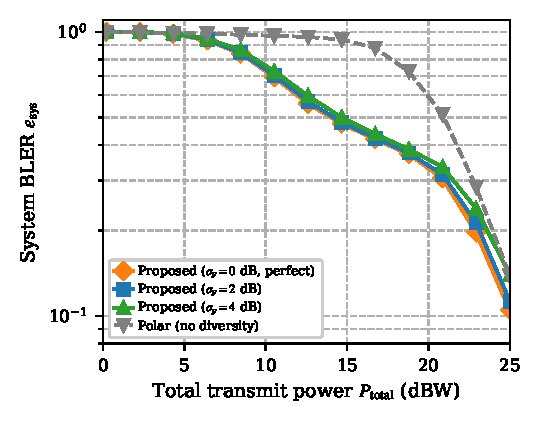
\includegraphics[width=0.7\columnwidth]{bler_robustness_prediction.eps}\\
{\small \textbf{Fig.~\ref{fig:bler_robustness}:} {\color{blue}System BLER versus total transmit power under imperfect prediction with combined prediction error $\sigma_p$.}}
\end{center}

\begin{center}
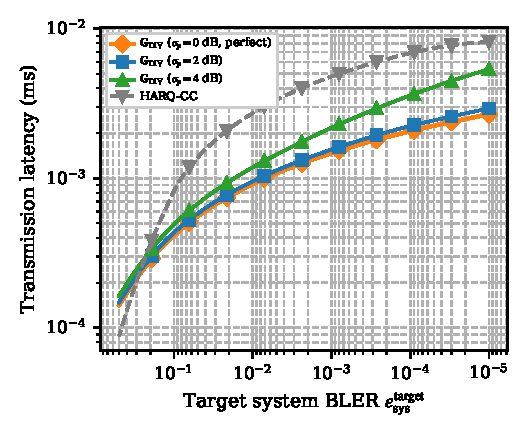
\includegraphics[width=0.7\columnwidth]{latency_robustness_prediction.eps}\\
{\small \textbf{Fig.~\ref{fig:latency_robustness}:} {\color{blue}Transmission latency versus target system BLER under imperfect prediction at $P_{\mathrm{total}} = 10$~dBW.}}
\end{center}

The ephemeris prediction targets a future frame at time $t_{k+\Delta}$ (Eq.~\eqref{eq:predicted_path_loss}). Since the total system latency $T_\Delta$ is on the order of milliseconds while LEO orbital geometry changes over tens of seconds, the prediction horizon contributes negligible additional mismatch relative to the $\sigma_p$ values studied above. In summary, the BLER degrades by only ${\sim}3$ percentage points at $\sigma_p = 4$~dB, and the latency advantage over HARQ-CC is preserved across all evaluated $\sigma_p$ values.

We trust that the robustness analysis and supporting figures address this concern.


\subsection{Reviewer Comment-6}



\begin{mdframed}
\begin{quote}

Integration Details of Diversity Transform and FEC \\
   The paper mentions using Polar codes as the FEC component but does not deeply explore the co-design with the diversity transform layer (e.g., rate allocation, decoder design). Relevant technical details should be supplemented.


\end{quote}

\end{mdframed}


\subsection{Response}

We thank the reviewer for this comment. The integration between the diversity transform and FEC is detailed in Sections~IV-B and~IV-C of the manuscript, and the revised version includes additional clarifications and a new FEC comparison figure. The co-design comprises three aspects: (i) decoupled rate allocation, where the FEC rate $R_c$ is chosen to match per-subchannel SNR while the MDS rate $\varrho/n_{\mathrm{out}}$ is determined by erasure tolerance, giving an effective end-to-end rate $R_{\mathrm{eff}} = R_c \cdot \varrho/n_{\mathrm{out}}$; (ii) a single-pass decoder architecture where the diversity demapper produces standard $N$-bit LLR vectors that feed directly into an unmodified SCL decoder, with reliability-aware LLR scaling bridging the two layers; and (iii) FEC-agnostic operation, confirmed by a new figure (Fig.~\ref{fig:fec_comparison}) showing that polar and LDPC codes achieve nearly identical BLER (gap $< 0.2$~dB) at all three code rates when combined with $\mathbf{G}_{\mathrm{DIV}}$. Regarding rate allocation, the diversity transform and FEC code operate at separate layers with independent rate parameters. The FEC code operates at rate $R_c = K/N$ (e.g., $R_c = 1/2$ for a $(256,128)$ polar code), while the diversity transform introduces a rate overhead of $\varrho/n_{\mathrm{out}}$ (e.g., $12/18 = 2/3$ for the $[6,4,3]$ MDS code), giving an effective end-to-end rate of $R_{\mathrm{eff}} = R_c \cdot \varrho/n_{\mathrm{out}}$. This decoupled rate allocation is a deliberate design choice: the FEC rate $R_c$ is chosen to match the per-subchannel SNR, while the MDS rate is determined by the number of subchannels that must be tolerated as erasures. In Section~IV-B:

\begin{quote}
``Polar codes are adopted as the FEC component owing to their capacity-achieving performance. The diversity transform operates as an inner outage-protection stage, while the polar code serves as the outer error correction component. Let $G_{\text{POL}}$ denote the generator matrix of an $(N,K)$ polar code, and let $G_{\text{DIV}} \in \mathbb{F}_2^{\varrho \times n_{\text{out}}}$ be the diversity transform constructed in Section~\ref{sec:diversity_transform_construction}. For a polar input matrix $U$, the combined encoding operation is
$Z = G_{\text{DIV}}^{\mathsf{T}}\, U\, G_{\text{POL}},$
where $Z$ contains the $n_{\text{out}}$ transform outputs to be mapped onto the fixed set of NTN subchannels. Vectorising both sides gives $ z = u\left(G_{\text{POL}} \otimes G_{\text{DIV}}\right),$ where $u$ and $z$ are the vectorised forms of $U$ and $Z$, and $G_{\text{PD}} = G_{\text{POL}} \otimes G_{\text{DIV}}$ is the combined polar--diversity generator. Since $G_{\text{DIV}}$ is rectangular with $n_{\text{out}} > \varrho$, the composite matrix $G_{\text{PD}}$ is also rectangular, thereby embedding the desired redundancy directly into the transform domain. $\ldots$ {\color{blue} Each information subword is independently encoded into a polar codeword of length $N$. Accordingly, the channel-coding blocklength used in the finite-blocklength analysis of Section~\ref{sec:finite blocklength} is $n_c = N$, with each codeword occupying $N$ binary-modulated channel uses. For each subchannel, the OTFS frame contains $N_{\mathrm{D}} \times M_{\mathrm{D}}$ resource elements and carries $(n_{\mathrm{out}}/n_{\mathrm{s}})$ independently encoded transform outputs. This establishes the
interface between the diversity transform layer and the OTFS physical layer.}''
\end{quote}

Regarding decoder design, the receiver performs diversity demapping and FEC decoding in a single pass, as detailed in Section~IV-C. The full rank guarantee of Theorem~\ref{thm:block_mds} ensures that the system of equations is solvable whenever the number of surviving subchannels meets the MDS recovery threshold. In Section~IV-C:

\begin{quote}
``The received transform outputs from surviving subchannels form the linear system $\mathbf{Z}(E^c) = G_{\mathrm{DIV}}^{\mathsf{T}}(E^c)\,\mathbf{X}$, where $E^c$ denotes the set of surviving transform-output indices. By Theorem~\ref{thm:block_mds}, whenever $|\mathcal{J}(E)| \geq k_{\mathrm{c}}$ the submatrix $G_{\mathrm{DIV}}(E^c)$ has full row rank $\varrho$, and the encoder subword matrix $\mathbf{X}$ is uniquely recoverable via the binary left inverse $G_{\mathrm{DIV}}^{\dagger}(E^c)$, which can be precomputed offline for all anticipated erasure patterns in $\mathcal{E}_{\mathrm{robust}}$. For soft-decision decoding, the demapper computes max-log maximum a posteriori (MAP) log-likelihood ratios (LLRs) from the channel outputs in a single pass, jointly marginalizing over all $2^{\varrho}$ input hypotheses. $\ldots$ The LLR is $\ldots$ scaled by the instantaneous subchannel reliability score obtained from the receiver's local channel estimate:
$\Lambda_i^{(j)} \leftarrow \hat{\eta}_i \cdot \Lambda_i^{(j)},$
where $\hat{\eta}_i = 1 - \epsilon_i(\hat{\gamma}_i^{\mathrm{E2E}}, n_i, R)$ is evaluated from the receiver-estimated end-to-end SNR $\hat{\gamma}_i^{\mathrm{E2E}}$ using the finite-blocklength error probability of~\eqref{eq:bler_cdf_combined}. This instantaneous per-subchannel reliability estimate is computed locally at the receiver using only its own channel estimation results. {\color{blue}The demapper output is a vector of $N$ soft LLRs corresponding to the polar-coded bits. These LLRs are passed to a single successive cancellation list (SCL) polar decoder that recovers all $K$ information bits from the original $(N,K)$ polar code in one forward pass. No modification to the standard SCL algorithm is required.} The combined polar--diversity generator $G_{\mathrm{PD}} = G_{\mathrm{POL}} \otimes G_{\mathrm{DIV}}$ preserves the algebraic rank guarantees throughout the decoding process without requiring bit-level interleaving.''
\end{quote}

The reliability-aware LLR scaling ensures that soft information from degraded subchannels is appropriately downweighted before entering the FEC decoder, preventing unreliable observations from corrupting the decoding process.

Regarding FEC-agnostic operation, the revised manuscript includes a new FEC comparison figure (Fig.~\ref{fig:fec_comparison}) demonstrating that the framework is not restricted to polar codes. In Section~\ref{sec:results}:

\begin{quote}
``{\color{blue}Fig.~\ref{fig:fec_comparison} demonstrates the FEC-agnostic operation of the proposed diversity transform by comparing polar codes (SCL decoding, list size~$32$) and LDPC codes (BP decoding, $50$ iterations) at three code rates $R_c \approx 1/4$, $1/2$, and $3/4$. All codes are combined with the diversity transform $\mathbf{G}_{\mathrm{DIV}}$ and evaluated under identical channel conditions. At each code rate, the polar and LDPC curves are nearly indistinguishable, with the residual gap remaining below $0.2$~dB across the entire power range. This confirms that the system BLER is dominated by the diversity transform's erasure recovery mechanism rather than by the specific FEC decoder, confirming FEC-agnostic operation. The diversity gain is largest at higher code rates: at $R_c = 3/4$, the no-diversity baseline remains above $0.25$ even at $P_{\mathrm{total}} = 23$~dBW, whereas the diversity-transform-equipped schemes reach $0.03$, because the weaker FEC protection makes the system more reliant on the erasure recovery provided by $\mathbf{G}_{\mathrm{DIV}}$. At $R_c = 1/4$, the stronger FEC narrows the gap, but the diversity transform still provides a consistent advantage across all power levels.}''
\end{quote}

\begin{center}
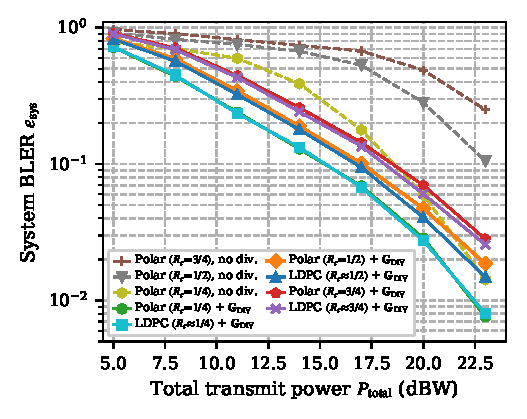
\includegraphics[width=0.7\columnwidth]{fec_comparison.eps}\\
{\small \textbf{Fig.~\ref{fig:fec_comparison}:} {\color{blue}System BLER versus total transmit power for polar and LDPC codes with the proposed diversity transform. No-diversity baselines shown for reference.}}
\end{center}

In summary, the co-design operates through decoupled rate allocation between the FEC layer ($R_c$) and the MDS diversity layer ($\varrho/n_{\mathrm{out}}$), reliability-aware LLR scaling at the demapper that bridges the diversity and FEC stages, and the combined generator $G_{\mathrm{PD}} = G_{\mathrm{POL}} \otimes G_{\mathrm{DIV}}$ that preserves the algebraic rank guarantees throughout decoding. The FEC comparison in Fig.~\ref{fig:fec_comparison} validates that this architecture is FEC-agnostic, with polar and LDPC codes achieving nearly identical performance at all code rates.

We trust that these details clarify the co-design between the diversity transform and FEC.


\subsection{Reviewer Comment-7}



\begin{mdframed}
\begin{quote}

Limitations of System Latency Analysis \\
   The manuscript discusses overall latency but overlooks the impact of latency discrepancies between different sub-channels on the performance of the diversity transform. Further analysis on adaptability in asynchronous transmission scenarios is recommended.


\end{quote}

\end{mdframed}


\subsection{Response}

We thank the reviewer for this comment. The latency discrepancies between subchannels arise from different slant ranges, resulting in differential propagation delays. In the revised manuscript, a new paragraph in Section~IV-F addresses block-level synchronisation: the differential delays are pre-compensated at the gateway through per-subchannel timing advance using ephemeris-derived slant ranges, following the standard 3GPP NTN procedure. The diversity transform operates at the block level and requires only that complete OTFS frames from surviving subchannels are available before demapping. Any residual timing offset ($< 1~\mu$s) is absorbed by the cyclic prefix. If timing failures prevent frame alignment on some subchannels, those are treated as erasures and recovered by the MDS guarantee of Theorem~\ref{thm:block_mds}. The effective latency is the maximum single-path delay, not the sum. The total system latency is defined in Section~IV-D:

\begin{quote}
``Regarding latency, the end-to-end delay comprises three
components: $T_{\Delta} = T_{\mathrm{prop}} + T_{\mathrm{frame}}
+ T_{\mathrm{proc}},$
where $T_{\mathrm{prop}}$ is the one-way propagation delay,
$T_{\mathrm{frame}} = n_c/(M_{\mathrm{D}}\Delta f)$ is the OTFS
frame duration, and $T_{\mathrm{proc}}$ represents the processing
delay at the gateway, satellite, and user equipment, which is
negligible relative to propagation delay. $\ldots$
Since all $n$ subchannels are transmitted simultaneously within
a single OTFS frame, the total latency $T_{\Delta}$ remains
independent of $n$. The algebraic recovery guarantee of
Theorem~\ref{thm:block_mds} ensures correct decoding within a
single OTFS frame with no feedback or retransmission overhead.''
\end{quote}

In Section~IV-F, we now write:

\begin{quote}
``{\color{blue}Regarding block-level synchronisation across subchannels, the diversity transform operates on the algebraic data plane at the gateway, mapping encoded subwords to transform outputs before transmission. The differential propagation delays between the gateway and each satellite are deterministic functions of the ephemeris-derived slant ranges in~\eqref{eq:slant_range} and are pre-compensated at the gateway through per-subchannel timing advance, following the standard 3GPP NTN timing advance procedure~\cite{3GPP38821}. Consequently, the OTFS frames arriving at the UE from different satellites are block-aligned, and the diversity transform construction is independent of the physical-layer timing.}''
\end{quote}

For a LEO constellation at $550$~km altitude, the maximum differential delay between two co-visible satellites is approximately $2$--$4$~ms, depending on the elevation spread. The diversity transform operates at the block level and mixes entire coded subwords ($N = 256$ bits each) across subchannels, so it requires only that complete OTFS frames from all surviving subchannels are available at the receiver before demapping begins. Any residual timing offset after TA pre-compensation (typically $< 1~\mu$s) is absorbed by the OTFS cyclic prefix. Even if one or more subchannels experience timing failures that prevent frame alignment, the diversity transform treats these subchannels as erasures. The MDS recovery guarantee of Theorem~\ref{thm:block_mds} ensures full data recovery as long as at least $k_{\mathrm{c}}$ subchannels deliver correctly aligned frames, providing inherent robustness to asynchronous scenarios without requiring any modification to the diversity transform design.

Since the gateway pre-compensates the differential delays, the effective latency seen by the diversity transform is the maximum single-path propagation delay, not the sum. Corollary~\ref{cor:latency_reduction} confirms that the minimum blocklength required by the diversity transform satisfies $n_c^{*}(\epsilon^*, \gamma) < n_c^{*}(\epsilon_{\mathrm{sys}}^{\mathrm{target}}, \gamma)$ and decreases monotonically as the number of subchannels or the MDS minimum distance increases.

We trust that the timing advance discussion and latency analysis resolve the concern about inter-subchannel latency discrepancies.


\subsection{Reviewer Comment-8}



\begin{mdframed}
\begin{quote}

Feasibility of Practical Deployment \\
   The compatibility of the proposed diversity transform with existing satellite communication standards (such as 3GPP NTN) is not addressed. A discussion on standardization and practical deployment is advised.


\end{quote}

\end{mdframed}


\subsection{Response}

We thank the reviewer for this suggestion. In the revised manuscript, a new deployment paragraph has been added at the end of Section~IV-F. The proposed diversity transform is compatible with the 3GPP NTN framework: it operates entirely at the gateway side using the transparent bent-pipe relay architecture from TR~38.821, requires no satellite payload modification, and adds only a soft-decision diversity demapper at the UE with negligible overhead. The ephemeris-driven prediction uses orbital data already broadcast in NR-NTN system information, and the FEC-agnostic design ensures compatibility with both polar codes (5G NR control channels) and LDPC codes (5G NR data channels). In the revised manuscript:

\begin{quote}
``{\color{blue}From a practical deployment perspective, the proposed diversity transform is compatible with the 3GPP NTN framework. The transform operates entirely at the gateway side, requiring no modification to the satellite payload (which remains a transparent bent-pipe relay) or to the UE physical-layer processing beyond the addition of a soft-decision diversity demapper. The ephemeris-driven prediction relies on satellite orbital data already broadcast in the NR-NTN system information~\cite{3GPP38821}, and the per-subchannel timing advance follows the standard 3GPP NTN procedure. The FEC-agnostic design ensures compatibility with both polar codes (5G NR control channels) and LDPC codes (5G NR data channels), enabling integration into existing NR-NTN protocol stacks without cross-layer redesign.}''
\end{quote}

We trust that the new deployment paragraph clarifies the compatibility with 3GPP NTN.


\subsection{Reviewer Comment-9}



\begin{mdframed}
\begin{quote}
Citation Completeness of Related Work \\
   The paper cites several works on OTFS and finite blocklength analysis; however, regarding channel estimation—particularly near-field XL-MIMO channel estimation in low SNR scenarios—the following recent study could be referenced:"Enhanced Polar-Domain Channel Estimation for Near-Field XL-MIMO in Low-SNR Scenarios." This work proposes innovative methods for channel estimation in massive MIMO systems and is strongly relevant to the theme of reliability enhancement in high-dynamic channels discussed in this manuscript. Citing it would enrich the discussion of related work. 



\end{quote}

\end{mdframed}


\subsection{Response}

We thank the reviewer for this suggestion. The recommended reference~\cite{Wang2025PolarXLMIMO} has been cited in the revised manuscript in the introduction, where the challenges of CSI acquisition in satellite systems with large antenna arrays are discussed:

\begin{quote}
``$\ldots$ which significantly increases the CSI overhead~{\color{blue}\cite{Wang2025PolarXLMIMO}}.''
\end{quote}
\vskip 0.2in
We are grateful for your careful and detailed review. Your comments have helped us significantly improve the practical relevance and technical completeness of the manuscript. We hope that the revisions address all concerns and look forward to your further consideration.
%%%%%%%%%%%%%%%%%%%%%%%%%%%%%%%%%%%%%%%%%%%%%%%%%%%%%%%%%%%%%%%%%%%%%%